The \textbf{DICOM File Format} decribes how the information, encapsulated in an  \textbf{SOP instance}, should be stored in a byte stream, in a file on a physical medium. Each DICOM file is composed of two instance: a \textbf{Header} followed by a \textbf{Data Set}.

\begin{itemize} 
\item \textbf{The Header} contains 128 bytes preamble (which are all set to zero if it is not used) followed by 4 byte DICOM prefix (DICM). The header is not necessary included in the file but is useful to make access to data easier, indeed the prefix allows to quickly acknowledge DICOM format. Besides, no structure is required for the preamble.  

\item \textbf{The Data Set} is organised as consecutive \textbf{DICOM Data Element} (or Data Attribute), referenced in the DICOM standard [10]. Those Data Element can represent various information, from the patient name and birth to theimage pixels. More precisely one \textbf{DICOM Data Element} is \textit{one unit of information} corresponding to one encoded \textbf{Information Object Definition (IOD) Attribute}, defined above. Figure 4 gives a representation of the DICOM File structure.
\end{itemize}

\begin{figure}[ht]
\centering
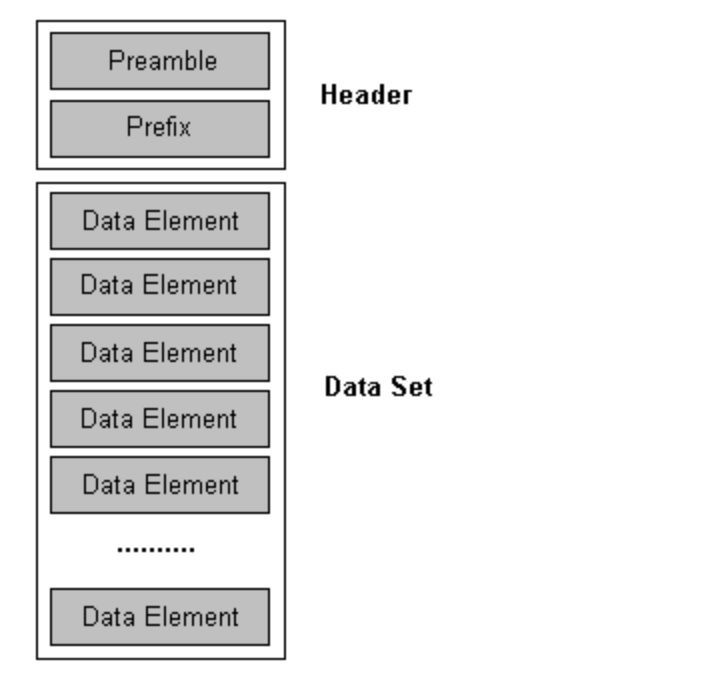
\includegraphics[width = 0.45\hsize]{./figures/DicomFileFormat}
\caption{Basic DICOM File Structure}
\end{figure}

\newline \vspace{5mm}
\textbf{DICOM Data Element} are \textit{Tag Element}, therefore DICOM can be said to be a tag file format, this mean that each element is referenced by a unique \textbf{Tag Number} defining the element and its properties. In the Data Set, Data Elements are ordered by increasing Tag Number. Each Data Element is made of the same range of consecutive fields: 
\begin{itemize} 
\item \textbf{Tag Number}: it consists in an ordered pair of 16 bits unsigned integer of the form (gggg,eeee)  representing the \textit{Group Number} - defining the Information Entity - followed by the \textit{Element Number} - defining the attribute. For example, in the tag (0028,0010), the Group Number is 0028 and correspond to the Image group, the Element Number is 0010 and correspond to the row (especially to the length of the image in pixels).
\item \textbf{Value Representation}: it defines the data type of the element. As the Tag Number already implies the data type, the value representation can be omitted.
\item \textbf{Value Length}: either 16 or 32 bits element, this defines the length of the following value.
\item \textbf{Value Field}: consists in an even number of bytes containing the value of the element; this field can contain the Value Multiplicity, which would specified the number of values that can be encoded in the field. 
\end{itemize}

\begin{figure}[ht]
\centering
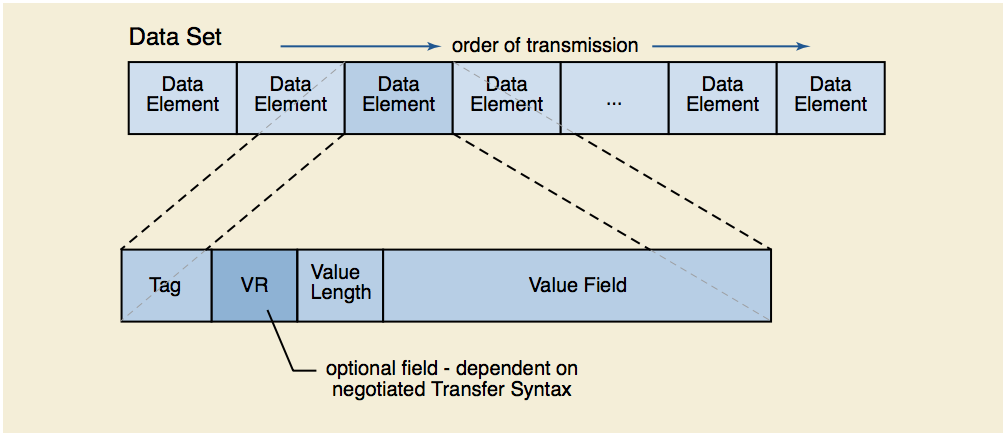
\includegraphics[width = 0.8\hsize]{./figures/DataSetandDataElement}
\caption{Data Set and Data Element structure}
\end{figure} 

